%%%%%%%%%%%%%%%%%%%%%%%%%%%%%%%%%%%%%%%%%%%%%%%%%%%%%%%%%%%%%%%%%
%%%   Describing and Contextualizing Events in TV News Show   %%%
%%%%%%%%%%%%%%%%%%%%%%%%%%%%%%%%%%%%%%%%%%%%%%%%%%%%%%%%%%%%%%%%%

% THIS IS SIGPROC-SP.TEX - VERSION 3.1
% WORKS WITH V3.2SP OF ACM_PROC_ARTICLE-SP.CLS
% APRIL 2009
\documentclass{sig-alternate}

\newcommand{\superscript}[1]{\ensuremath{^{\textrm{#1}}}}

\usepackage{url}
\usepackage{textcomp}
\usepackage{color}
\usepackage{listings}
\usepackage{multirow}
\usepackage{mathtools}
\usepackage{graphicx}
\usepackage{fancyvrb}
\usepackage{amsmath}
\usepackage{graphicx}
\usepackage[font=small,labelfont=bf]{caption}
\setcounter{MaxMatrixCols}{20}
\usepackage{pbox}

% listing styles
\lstset{numbers=left, numberstyle=\tiny,basicstyle=\ttfamily\scriptsize, tabsize=2, keywordstyle=\underbar, stringstyle=\small, backgroundcolor=\color[gray]{0.94}, framexleftmargin=2pt}
\lstdefinestyle{rdfa}{numberblanklines=true, morekeywords={}}

% Turtle box
\definecolor{olivegreen}{rgb}{0.2,0.8,0.5}
\definecolor{grey}{rgb}{0.5,0.5,0.5}
\lstdefinelanguage{ttl}{
sensitive=true,
morecomment=[l][\color{grey}]{@},
morecomment=[l][\color{olivegreen}]{\#},
morestring=[b][\color{blue}]\",
keywordstyle=\color{cyan},
morekeywords={version,owl,rdf,rdfs,xml,xsd,dbpedia,dbo,str,sso,scms,fr,ld}
}
\lstset{
        basicstyle=\ttfamily\scriptsize,
        upquote=true,
        showspaces=false,
        showstringspaces=false,
        showtabs=false,
        tabsize=2,
        frame=none,
        breaklines,
        numbers=none,
        framexleftmargin=2mm,
        xleftmargin=2mm,
}

\newcommand{\hilight}[1]{\colorbox{yellow}{#1}}
\newcommand{\todo}[1]{\colorbox{red}{#1}}

%%%%%%%%%%%%%%%%%%%%%%%%%%%%%%%
%%%  Beginning of document  %%%
%%%%%%%%%%%%%%%%%%%%%%%%%%%%%%%

\begin{document}

\title{Describing and Contextualizing Events in TV News Show}

\numberofauthors{5}
\author{
\alignauthor Jos\'e Luis Redondo Garc\'ia\\
	\affaddr{EURECOM}\\
	\affaddr{Biot, France}\\
	\email{redondo@eurecom.fr}
\alignauthor Laurens De Vocht\\
    \affaddr{Ghent University - iMinds}\\
    \affaddr{Ghent, Belgium}\\
    \email{laurens.devocht@ugent.be}
\alignauthor Rapha\"el Troncy\\
	\affaddr{EURECOM}\\
	\affaddr{Biot, France}\\
	\email{raphael.troncy@eurecom.fr}	\\
\and
\alignauthor Erik Mannens\\
    \affaddr{Ghent University - iMinds}\\
    \affaddr{Ghent, Belgium}\\
    \email{erik.mannens@ugent.be}
\alignauthor Rik Van de Walle\\
    \affaddr{Ghent University - iMinds}\\
    \affaddr{Ghent, Belgium}\\
    \email{rik.vandewalle@ugent.be}
}

\maketitle

%%%%%%%%%%%%%%%%%%
%%%  Abstract  %%%
%%%%%%%%%%%%%%%%%%

\begin{abstract}
Describing multimedia content in general and TV programs in particular is hard problem. Relying on subtitles to extract named entities that can be used to index fragments of a program is a common approach. However, this approach is limited to what is being said in a program and written in a subtitle lacking therefore a broader context. Furthermore, this type of index is restricted to a flat list of entities. In this paper, we combine the power of non-structured documents with structured data coming from DBpedia to generate a much richer, context aware metadata of a TV program. We demonstrate that we can harvest a highly precise context starting from named entities recognized in a TV fragment and we evaluate our approach on a TV news show.
\end{abstract}

% A category with the (minimum) three required fields
%\category{H.4}{Information Systems Applications}{Miscellaneous}
%A category including the fourth, optional field follows...
%\category{D.2.8}{Software Engineering}{Metrics}[complexity measures, performance measures]

%\terms{Theory}\textsl{}

%\keywords{ACM proceedings, \LaTeX, text tagging} % NOT required for Proceedings


%%%%%%%%%%%%%%%%%%
%%%  Introduction  %%%
%%%%%%%%%%%%%%%%%%

\section{Introduction}
\label{sec:introduction}

%Online media keeps increasing in scale and ubiquity, but it is currently still unstructured and badly connected to media of other formats or from other sources.
%[State of the Art: Named Entity Extraction, Expansion]
%[About LinkedTV?]
%LinkedTV is an integrated and practical approach towards experiencing Networked Media in the future Internet. This project aims to make multimedia content and Web information seamlessly interconnected. Technologically speaking, this vision requires systems to be able to represent multimedia information as is done in the Web of Data: described at different granularities and interlinked with other resources.
%Task like video
The amount of videos shared on the Web is constantly increasing. From a Semantic Web point of view those video segments need to be annotated with structured information and linked to other video segments. A new generation of innovative video services intend to use those semantic descriptions and media fragments for providing the users a television experience where multimedia content and Web information are seamlessly interconnected.

The annotation problem has been traditionally addressed by applying audiovisual techniques, like in \cite{ballan2011event}, but extracting semantic and structured content from a video is still more complex. One possible approach consist on using Named Entity Recognition (NER) over the textual information concerning a particular video fragment. Those techniques are an essential component of the Information Extraction domain that focus on: identifying atomic information units in texts, named entities; classifying entities into predefined categories (also called context types) by classification techniques and linking to real world objects using web identifiers (Named Entity Disambiguation). Various tools provide such computations, like AlchemyAPI\footnote{\fontsize{8pt}{1em}\selectfont \url{http://www.alchemyapi.com/}} or DBpedia Spotlight\footnote{\fontsize{8pt}{1em}\selectfont \url{http://spotlight.dbpedia.org/}}. If the textual information from the video includes temporal references (like in the case of the subtitles), it is possible to align the obtained entities with the time when they appear over video. Research initiatives like Katsiouli et al.~\cite{katsiouli2007} demonstrated that applying named entity recognition techniques in combination with domain ontologies on video subtitles achieves decent results in tasks like video classification.

For the Linked Data community, it is a first step to increase the volume of interconnected data. However from an exploitation point of view those promising techniques still introduce some issues. On the one hand, subtitles are not always complete enough to be the only textual source to rely on. The context around a particular event can be broader than what is transcribed from the video. On the other hand, a plain list of name entities can fail to characterize what is described in the multimedia content: sometimes we also need to know how important they seem to be regarding the event and how they related to each other. 

In this paper we present an approach for deeper annotating a news event video by alleviating the lack of textual resources that limits the application of semantic extraction techniques. We first extend the initial set of descriptions about the current event via Google searches and entity clustering. Secondly, we use an optimized pathfinding algorithm \cite{de2013discovering} implemented in the Everything is Connected Engine (EiCE).
%firstly introduced with the Everything is Connected (EiC) Demo at the \emph{ISWC`12 Boston} conference \cite{Sande12}.
Applying these algorithms to Linked Data facilitates: resolving complex queries that involve the semantics of the relations between resources, discovering relevant resources and context-sensitive filtering resources. Users control and define which kind of relations and types of resources really matter. Each path between the discovered resources has a semantic meaning can be traced back to the original configuration of the user and forms the basis of an explanation rather than a ranking. A major contribution in this approach is that it minimizes the size of the candidate pool of resources in order to optimize queries and increase the quality of the resulting paths.

%%%%%%%%%%%%%%%%%%
%%%  Approach  %%%
%%%%%%%%%%%%%%%%%%

\section{Approach}

To reconstruct the semantic context associated with one particular news video, we highlight the main concepts and entities involved and explain how they are related to each other. The complete processing workflow takes as input the textual transcript of a multimedia resource depicting the event, as well as the start and end date for which that particular event has been considered relevant. 

We assume additionally that the analyzed event has a minimal presence and coverage on the Web to ensure that the subsequent data mining techniques can collect sufficient data to reconstruct the event's context. The output of the algorithm is a pair $Context_{Event1}=\left [  \varepsilon , \rho \right ]$  where $\varepsilon$ is a list named entities together with a numeric relevance score ($ \varepsilon =\left \{ E\times \mathbb{R} \right \}$,  being $E$ named entities classified using the NERD ontology\footnote{\fontsize{8pt}{1em}\selectfont \url{http://nerd.eurecom.fr/ontology/nerd-v0.5.n3}}) and $\rho$ is a set of predicates $\left [ e_{1},e_{2}, p \right ]$, relating the aforementioned entities ($e_{1}\in E \vee  e_{2}\in E$).

Our hypothesis states that this knowledge representation of the events provides a sufficient source of information for satisfying the viewer's information needs and suports complex multimedia operations such as search and hyperlinking.

\subsection{Named Entity Extraction}

For each news item we perform named-entity recognition over the corresponding subtitles by using the NERD~\cite{Rizzo2012b} framework. The language of the considered videos is English but NERD supports many others. The output of this phase is a collection of entities annotated using the NERD Ontology v0.5, that comes with a first relevance score obtained from the considered extractors. This set includes a first set of ranked entities that are explicitly mentioned during the video. Other entity based video annotation tools~\cite{yunjia2013} stop at this point even when entities are still missing that can be relevant for the viewer in the context of the current event. We tackle this problem by extending this first list of concepts via the entity expansion component.

\subsection{Named Entity Expansion from Unstructured Resources}
\label{sec:expansion}

The set of entities obtained from a traditional named entity extraction operation is normally insufficient and incomplete for expressing the context of a News event. Sometimes some entities spotted over a particular document are not finally disambiguated because the textual clues around are not sufficient precise for the name entity extractor, while in other cases they are not even mentioned in the transcripts but are relevant for understanding the  story behind. This is an inherent problem in information retrieval tasks: a single description about the same resource does not necessarily summarize the whole picture about it.

The named entity expansion operation relies on the idea of retrieving and analyzing extra documents in the Web where the same event or the same part of the event is also described. By increasing the size of the sample we increase the completeness of the context and the representativeness of the proposed set of entities, reinforcing relevant entities and finding new ones that are potentially interesting inside the context of that news item.

The entire logic will further be described in the following subsections and mainly consist of (1) building an appropriate search query from the original set of entities, (2) retrieving extra documents about the same news event, and (3) analyzing them for providing a more complete and better ranked set of final entities, as illustrated in Figure~\ref{fig:namedEntityExpansion}.

\begin{figure}[h!]
\centering
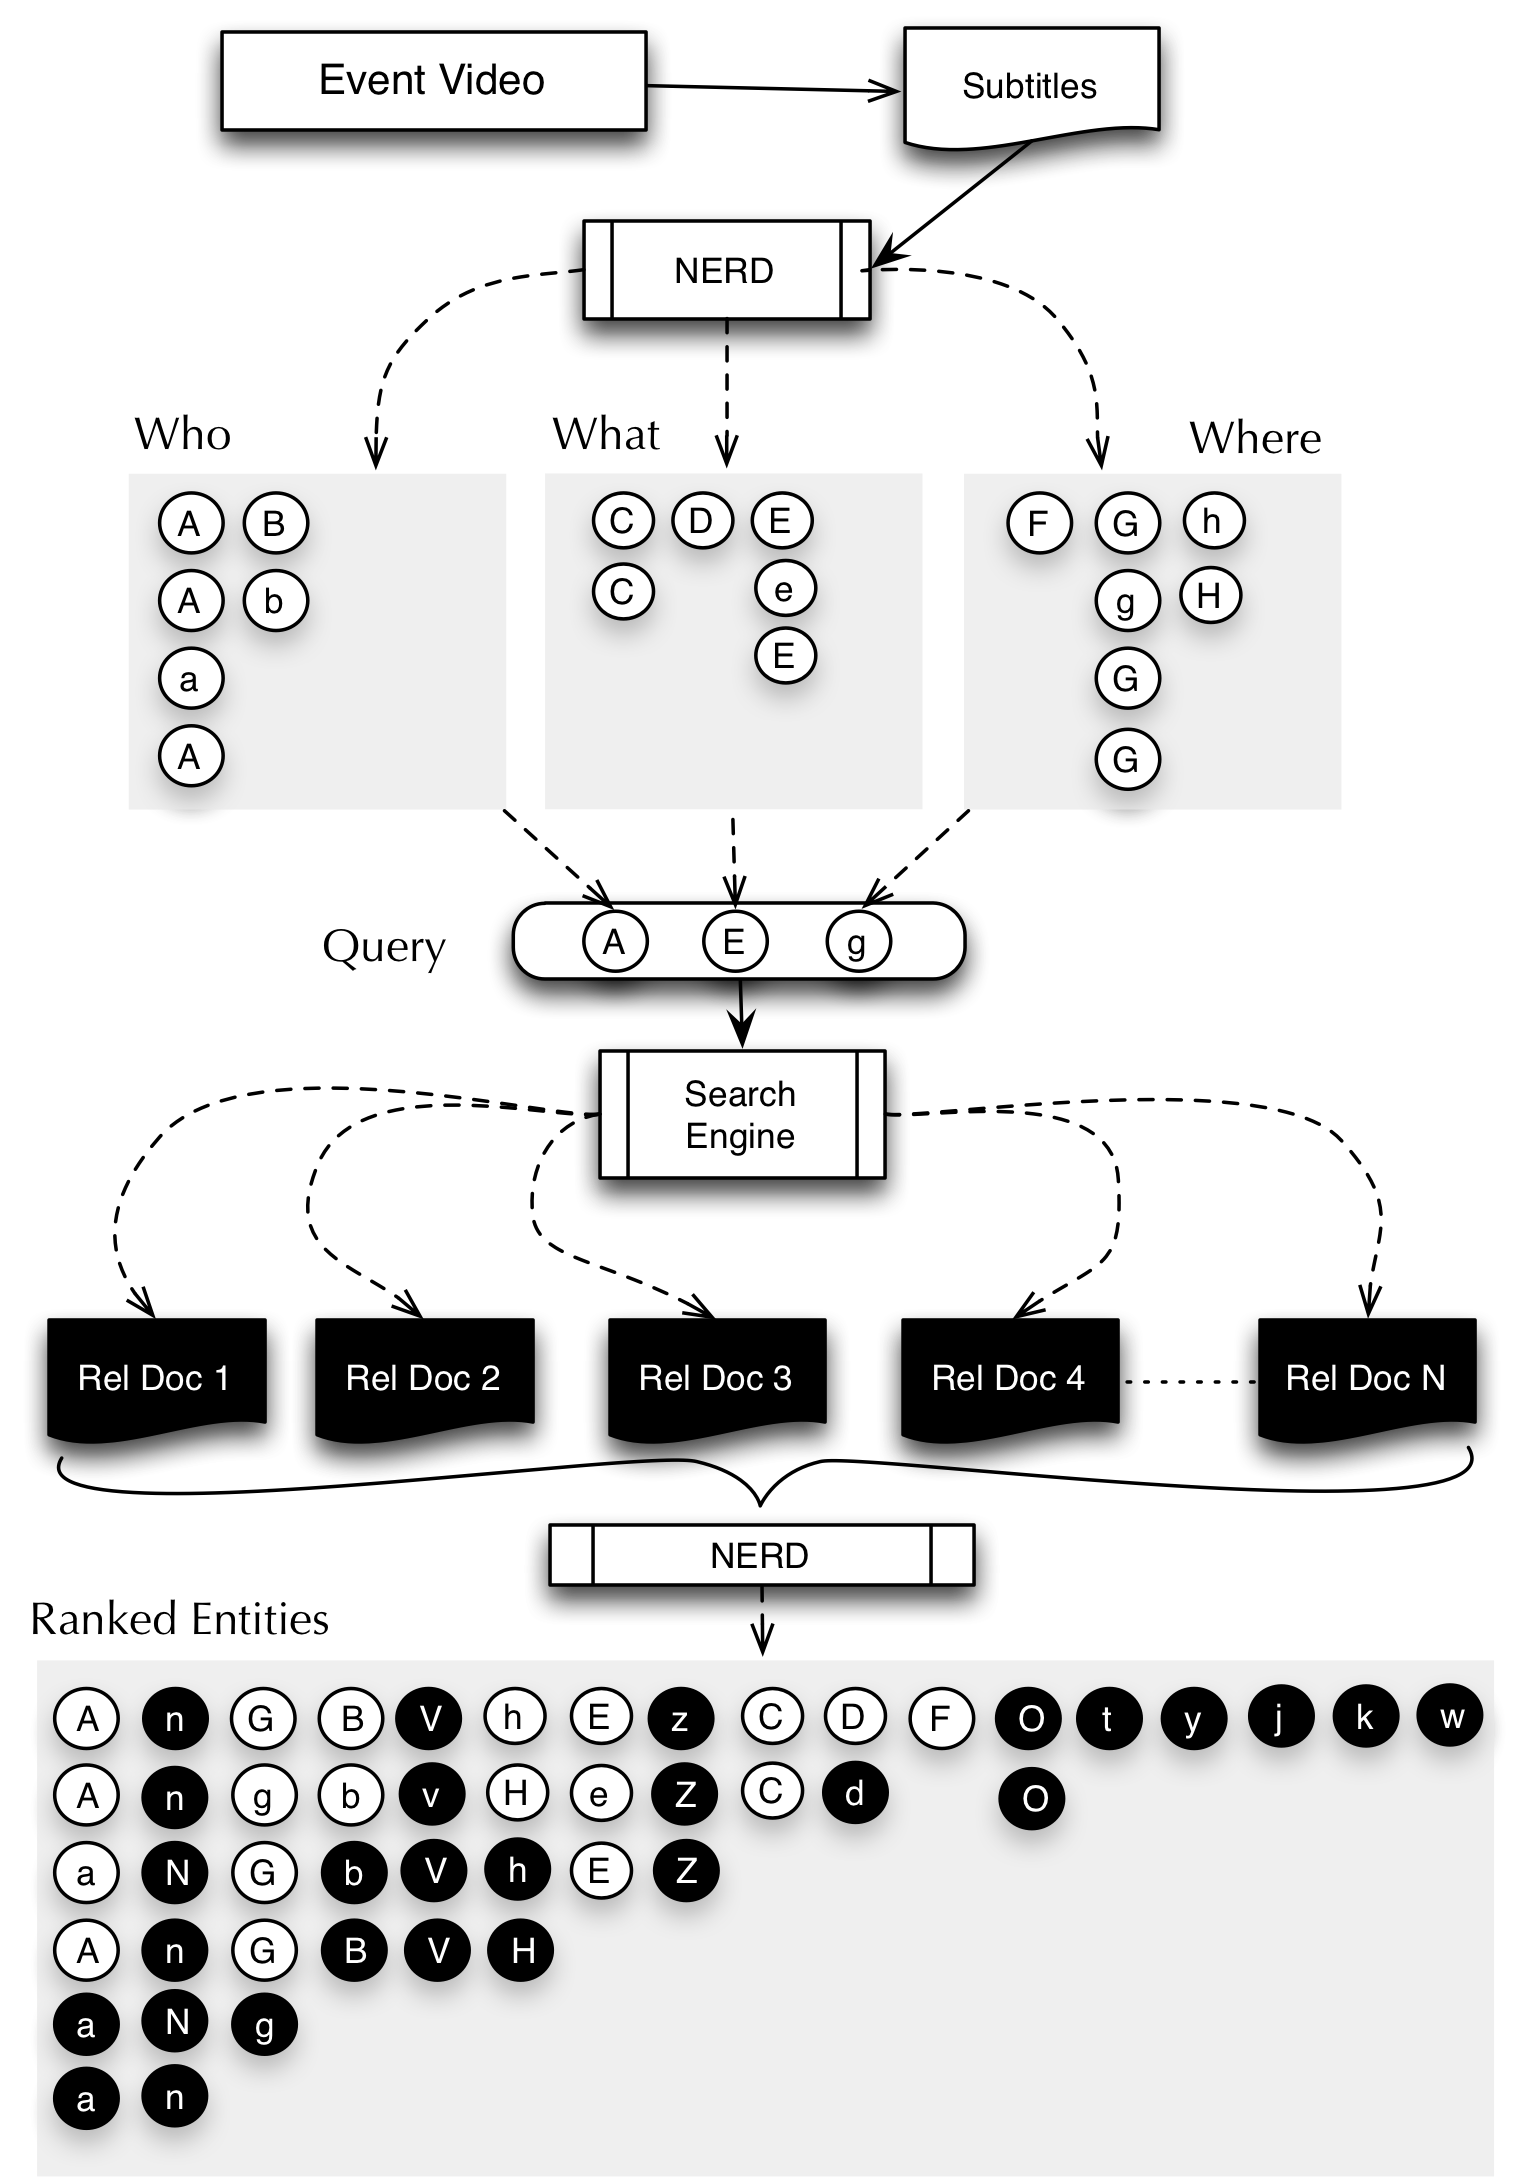
\includegraphics[width=0.4\textwidth]{figure/ExpansionDiagram}
\caption{Schema of Named Entity Expansion Algorithm.}
\label{fig:namedEntityExpansion}%\end{figure}
\end{figure}

\subsubsection{Query Generation}

The \emph{Five W's} is a popular concept of information gathering in journalistic reporting. It captures the main aspects of a story or incident: who, when, what, where, and why~\cite{LiJia2007}. We try to represent the news item in terms of four of those five W's (who is involved in the event, where the event is taking place, what the event is about, and when has happened) in order to generate a query that retrieves documents associated to the same event. 
%This is like a normal user would type in a Web search engine when looking for descriptive documents about the same news event.

Firstly the original entities are mapped to the NERD Core ontology, which considers 10 main classes: Thing, Amount, Animal, Event, Function, Organization, Location, Person, Product and Time. From these ten categories we generalize three classes: the Who from \url{nerd:Person} and \url{nerd:Organization}, the Where from \url{nerd:Location}, and the What from the rest of NERD types after discarding \url{nerd:Time} and \url{nerd:Amount} instances. The When or so-called temporal dimension does not need to be computed since it is provided by the video publisher as an inputs for this approach.

After generating the three sets of entities, the next step consist in ranking them in relevance according to a weighted sum of two different dimensions: their frequency in the transcripts and their former relevance scores coming from the named entity extractors. We have defined the function \emph{filterEntities(S)} for selecting the $n$ entities inside the set of entities $S$ whose relative relevance

\begin{equation}
R_{rel}\left ( e_{i}, S \right ) = R\left ( e_{i} \right ) / Avg \left ( R\left ( e_{i} \right )  \right )
\end{equation}

falls into the upper quarter of the interval

\begin{equation}
\left [ max\left ( R_{rel}\left ( e_{i}, S \right )  \right ) -min\left (  R_{rel}\left ( e_{i}, S \right ) \right ) \right ]
\end{equation}

The final query is a pair

\begin{equation}
\text{Query}_{Event} =\left [ \text{textQuery}, t \right ]
\end{equation}

where \textit{textQuery} is the result of concatenating the labels of the most relevant entities in the sets Who, What, Where in that particular order,
%\begin{equation}
%\begin{split}
%\textit{textQuery} = \text{labels} ( \text{filterEntities}(Who) \\ + \text{filterEntities}(What) \\ + \text{filterEntities}(Where) )
%\end{split}
%\end{equation}
and $t$ the time period dimension.
This query generation is depicted in the upper part of Figure~\ref{fig:namedEntityExpansion}. 
%For future research in the query construction technique we plan to directly use the Web resources themselves and not only their labels.

\subsubsection{Document Retrieval}

Once $\text{Query}_{Event}$ is built out of the original set of named entities it will be ready to be injected into a document search engine where additional descriptions about the news event can be found. In this situation, the kind of query generated in the previous step and the search engine chosen should be closely tied in order to maximize the quality of the obtained results. Of course the different behavior of search engines make some alternatives more suitable than others for certain kinds of events. The way the resulting documents change in the search engines for a particular kind of event is a research question that will not be studied in this paper.

In this paper we have resorted to Google Search REST API service\footnote{\fontsize{8pt}{1em}\selectfont  \url{http://ajax.googleapis.com/ajax/services/search/web?v=1.0}}  by launching a query with the text \textit{textQuery}. Due to quota restrictions imposed by Google, the maximum number of retrieved document is set to 30. However and according to the evaluation performed in Section~\ref{sec:evaluation}, this is enough for significantly extending the initial set of entities directly spotted by NERD.

Concerning the temporal dimension, we only keep the documents published in the time period $t+t_{e}$. We increase the original event period in $t_{e}$ because documents concerning a news event are not always published during the time of the action is taking place but some hours or days after. The value of $t_{e}$ depends on many factors like the nature of the event itself (it is a quick appearance in the media, or a deep fact with more repercussion) or the kind of documents the search engine is indexing (from very deep and elaborated documents that need time to be published, to light post generated by users in just some minutes). Based on the simple assumption that that longer event will provoke longer buzzes, we approximated  $t_{e} = t$, meaning that we consider also document published duration of the event.

The middle part of Figure~\ref{fig:namedEntityExpansion} shows this process. The query is inputted in the search engine to obtain other documents that elaborate on the same event from in the original video.Those documents (colored in black in the aforementioned Figure) will be further processed to increase the size of the collection and get extra insights about the news item.

\subsubsection{Entity Clustering}

In this phase the previously retrieved extra documents are now preprocessed and analyzed in order to extend and re-rank the original set of relevant entities and consequently get better insight about the studied event. Since most of the retrieved resources are Web pages, HTML tags and other annotations are removed, keeping only the main textual information. This plain text is then analyzed by the NERD framework in order to extract the named entities present.

In order to calculate the frequency of a certain resource inside the entire corpora, we group the different appearances of the same instance and check their cardinality. This is not a trivial task since the same entity can appear under different text labels, contain typos in the field or have different disambiguation URL's pointing to the same resource. We performed a centroid-based cluster operation over the instances of the entities. We considered the centroid of a cluster as the entity with the most frequent disambiguation URL's that also have the most repeated labels. As distance metric for comparing pairs of entities we applied strict string similarity over the URL's, and in case of mismatch, Jaro-Winkler string distance~\cite{winkler2006overview}
%TODO: Verify reference above
over the labels. The output of this phase is a list of clusters containing different instances of the same entity.

\subsubsection{Entity Ranking}

The final step of the expansion consists of ranking the different named entities obtained so far. To create this ordered list we assigned a score to every entity according to the following features: relative frequency of the entity in the transcripts of the event video; relative frequency of the entity over the extra document; and average relevance for the different instances according to the named entity extractors. The three dimensions are combined via a weighted sum where the relative frequency in the video subtitles has a bigger impact in the final score, followed by the relative frequency on the searched documents and the relevance from the extractors. The final output of the entity expansion operation is a list of entities together with their ranking score and the frequency in both the main video and in the collected extra documents.

%\begin{equation}
%\begin{split}
%E_{Expansion}\left (subtitles, timePeriod \right )= \\
%\left ( \left \{ e_{i},  relScore_{i}, Freq\left ( subtitles, e_{i} \right ), Freq\left ( extraDocs, e_{i} \right ) \right \} \right )
%\end{split}
%\end{equation}

Entities with a higher $relScore_{i}$ in the final classification are more representative for the context of the original. Also there are other advantages in the final set of results:
\begin{itemize}
  \item The bigger sample size leads to a better ranking. Entities appearing repeatedly in the extra documents will be promoted while those barely appearing will be pushed back to the end of the list.
  %TODO: documents? will have less relevance.
  \item Entities that originally have not been disambiguated can now have their corresponding URL if any of the similar instances appearing in the additional documents provide a link to a Web resource. The same occurs with incomplete or misspelled labels.
  \item  Finally, some entities ot mentioned in the original transcripts but important in the context of the event are now included in the list of relevant items since they have been spotted on the collected documents.
\end{itemize}

\subsection{Refining Event Context via DBpedia}

Once the set of context relevant entities has been expanded, we will use the knowledge from structured sources to reinforce the important entities and finding relevant predicates between them.

\subsubsection{Generating DBpedia paths}
\label{sec:dbpedia_path}

Before we filter the relations between resources to reinforce important entities, the candidate resources to be included in relations are pre-ranked. They are pre-ranked according to ``popularity'' and ``rarity'' essential components in the original PageRank algorithm \cite{page1999pagerank} and is used to sort candidate related nodes in the EiCE. The implementation of the EiCE takes the relations in to account by making use of the Jaccard coefficient to measure the dissimilarity and assign random walks based weight able to highly rank more rare resources, and guaranteeing that paths between resources prefer specific relations and not general ones \cite{moore2012novel}.

\begin{figure}[h!]
\centering
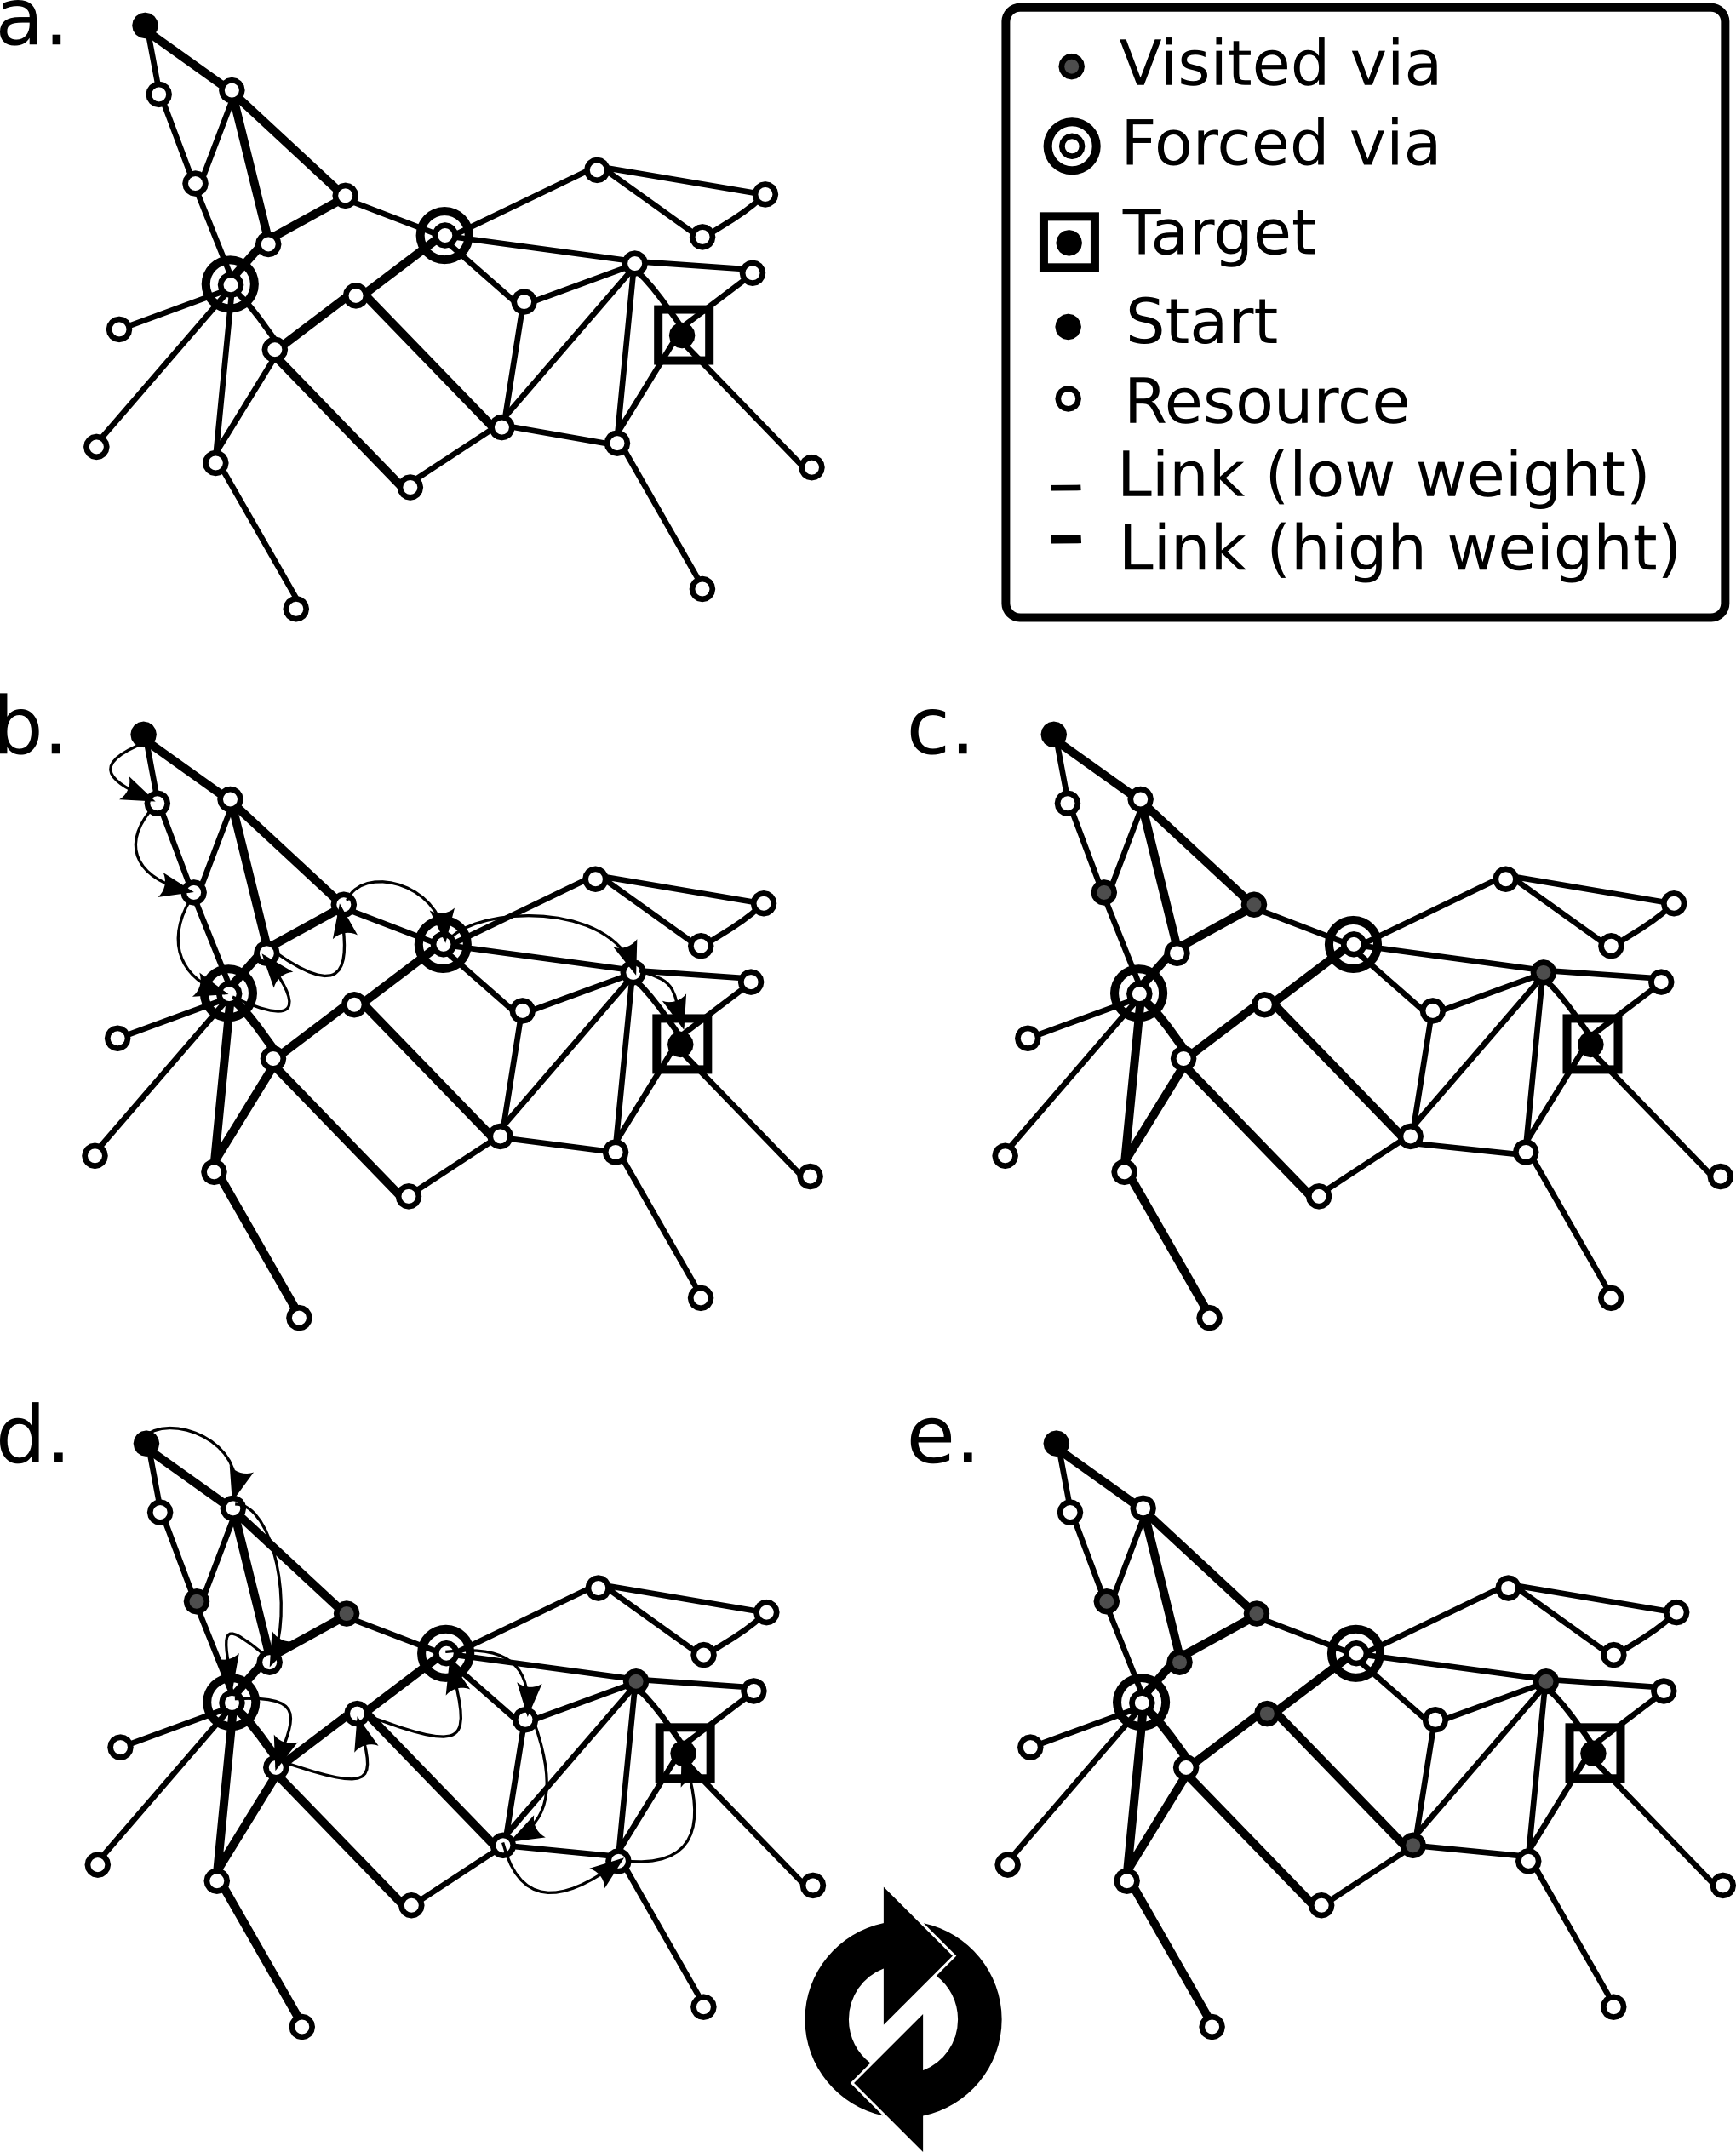
\includegraphics[width=0.4\textwidth]{graphmultipatternmatching.png}
\caption{Pattern matching with multiple results using an iterative pathfinding process.}
\label{fig:patternmatching}
\end{figure}

We pass on the main start resource, the target and via points. Figure~\ref{fig:patternmatching} shows the iterative process for generating the DBpedia paths. An initial state is computed in step \ref{fig:patternmatching}a. There are low weights and high weights
%, for the example 1 and 2 respectively
. Based on the weights of the links each path through the vias is optimized, so a path with the lowest total weight will be selected first, until the vias are added to the exclude list. The path from start to end is forced through the given via points (\ref{fig:patternmatching}b). This leads to additional visited resource as via points (\ref{fig:patternmatching}c). They occur because each computed path starts both from the start and the target resources and goes through the via points. The resources where they converge to each other are considered as new via points. These additional via points are included in the paths and therefore marked as visited. This is to make sure that in the next iteration, paths will go around the visited via (\ref{fig:patternmatching}d). The next paths are being computed over and over (\ref{fig:patternmatching}e) until a threshold number of paths is found and the context is large enough or when it takes to long to compute the next path (out of range). The final set of optimized paths is used for the context expansion.

\subsubsection{Analyzing Context Relevant Paths}

In this step the DPpedia path finding technique implemented in ~\ref{sec:dbpedia_path} is applied over the set of entities obtained via entity expansion. Since this list is too broad we need to establish in first place a division between what we consider \textit{MainEntities}(entities whose relative scores fall under the higher 25\% of the relevance range), and the \textit{additionalEntities}(the rest of entities in $E_{Expansion}$).

%in \url{demo.everythingisconnected.be/relations?uris=}
Afterwards, we calculate paths between all the possible pairs inside the set\textit{MainEntities}.
%following the REST methods exposed at \footnote{\url{demo.everythingisconnected.be/relations?uris=}}.
Once all the possible paths have been retrieved, we perform various analysis for detecting which are the most frequent classes and predicates:
\begin{itemize}
  \item  We detect the most frequent nodes ($F_{nodes} = f_{max}(n_{i})$ in $Paths (mainEntities)$).
  \item  We detect the most frequent predicates ($F_{prop} = f_{max}(p_{i})$ in $Paths (mainEntities)$). The edges (DBpedia properties) will determine which are the most relevant properties taking part in the context of this news item.
  \item  We study the connectivity between nodes (Adjacency Matrix $M_{i,j}$ where the distance between $e+{i}$ and $e+{j}$ is the average length of the paths linking them ($m_{i,j} = \\ Avg (lenght(Paths(e_{i}, e_{j})))$)
\end{itemize}

The output of this phase is a re-ranked list of entities from the expansion entity set based on the found DBpedia insights, the most important predicates and nodes inside the paths between pairs in $mainEntities$, and the adjacency matrix.

\begin{equation}
\begin{split}
\{Entities_{Extension + DBpedia}, E_{Expansion}, F_{nodes}, F_{prop}, M_{i,j} \} \\
\end{split}
\end{equation}

In the future, we plan to use the frequency measures about predicates available in $F_{prop}$ in order to more precisely rank the named entities. By applying the \textit{commonalities} REST function (\url{http://demo.everythingisconnected.be/commonalities?between=resource1&and=resource2&allowed=property})over the $mainEntities$ inside $Entities_{Extension + DBpedia}$, and for the properties with highest $F_{prop}$, we obtain the set of entities directly related with the original ones through the top predicates. Once more, the most frequent entities in Commonalities could promote the already existing entities in $Entities_{Extension + DBpedia}$.
%\url{http://demo.everythingisconnected.be/commonalities?between=http://dbpedia.org/resource/Lyon&and=http://dbpedia.org/resource/France&allowed=http://purl.org/dc/terms/spatial}

%%%%%%%%%%%%%%%%%%
%%%  Use Case  %%%
%%%%%%%%%%%%%%%%%%

\section{Use Case: Snowden Assylum}

We have applied the proposed method over a real scenario corresponding to the news video \url{http://www.bbc.co.uk/news/world-europe-23339199}, from the BBC News Europe Web site. The main story behind this media content is the request of asylum made by Edward Snowden to the Russian government. In an airport in Moscow, he publicly express his desire to obtain political help while he can find a safe way to reach the Latin American countries that offer a safe harbor. The time period for which this particular event is relevant goes from 2013-07-06 to 2013-07-17.

\subsection {Named Entity Extraction}

In a first step, Name Entity Extraction techniques are applied over the video transcript by using NERD. Below we show the list of entities directly extracted via this procedure, which brings a first approximation to the context of the news media item.

\begin{table}[tbp]
  \resizebox{8cm}{!} {
\begin{tabular}{ c | c | c | c | c }
  \hline     
 Label & Relevance & Sentiment & Type & URI  \\ \hline  
Russia & 0.809216 & Mixed & Location & DBpedia:Russia \\
Edward Snowden & 0.717369 & Mixed & Person & DBpedia:/Edward\_Snowden \\
South America & 0.56586 & Mixed & Location & DBpedia:South\_America \\
president Putin & 0.459811 & positive & Person & DBpedia:Vladimir\_Putin \\
president & 0.401138 & negative & JobTitle & DBpedia:President \\
Moscow & 0.352101 & Mixed & City & DBpedia:Moscow \\
CIA & 0.334887 & neutral & Organization & DBpedia:CIA \\
Bolivia & 0.324607 & neutral & Location & DBpedia:Bolivia \\
Obama & 0.321901 & negative & Person & DBpedia:Barack\_Obama \\
  \hline  
\end {tabular} 
  }
\caption{Result from Named Entity Extraction in NERD}
\end{table}

\subsection {Named Entity Expansion}

In a second step, the original set of entities is expanded as described in Section~\ref{sec:expansion}. The query generated for retrieving extra documents has the text "Edward Snowden asylum Russia", and is bounded to the period from 2013-07-06 to 2013-07-28. After analyzing the extra documents the  instances are re-ranked according to their global frequency. 

%\url{curl -X POST --data-binary @snowden.txt "http://localhost:8006/api/rankedentities?startdate=2013-07-16&enddate=2013-08-15&limit=50" --header "Content-Type:text/xml" -v >> snowden_textrazor_50_130716_130815.json2}

\begin{table}[tbp]
  \resizebox{8.5cm}{!} {
\begin{tabular}{ c | c | c | c | c | l }
  \hline     
Label & Relevance & $F_{video}$& $F_{Docu}$ & Type & URI \\ \hline                  
Russia & 1.0 & 7 & 264 & Location & DBpedia:Russia \\
Edward Snowden & 0.80479 & 2 & 227 & Person & http://dbpedia.org/resource/Edward\_Snowden \\
US & 0.61643 & 5 & 160 & Location & DBpedia:United\_States \\
Vladimir Putin & 0.39383 & 1 & 111 & Person & DBpedia:Vladimir\_Putin \\
asylum & 0.32876 & 4 & 80 & Thing & DBpedia:Right\_of\_asylum \\
Barack Obama & 0.31506 & 1 & 88 & Person & DBpedia:Barack\_Obama \\
Moscow, Russia & 0.30479 & 1 & 85 & Location & DBpedia:Moscow \\
American president & 0.19178 & 2 & 48 & Thing & DBpedia:President\_of\_the\_United\_States \\
Central Intelligence Agency & 0.19178 & 0 & 56 & Location & DBpedia:Central\_Intelligence\_Agency \\
Anatoly Kucherena & 0.147260 & 0 & 43 & Person & -- \\
extradition & 0.116438 & 2 & 26 & Thing & DBpedia:Extradition \\
White House & 0.10616 & 0 & 31 & Location & DBpedia:White\_House \\
Sheremetyevo & 0.0890 & 0 & 26 & Location & DBpedia:Sheremetyevo\_International\_Airport \\
WikiLeaks & 0.08219 & 0 & 24 & Organization & DBpedia:WikiLeaks \\
Washington's & 0.075342 & 0 & 22 & Location & DBpedia:Washington,\_D.C. \\
  \hline  
\end {tabular} 
  }
\caption{Top entities obtained via Named Entity Expansion}
\end{table}

The final result after the expansion operation is a bigger list of entities (over 100). In some cases, the previously spotted entities (like \textit{Extradition}) have been promoted in the hierarchy while others (like \textit{Right\_of\_asylum\\}) have been discovered in the new documents. For this use case, we have taken only a fixed number of top entities ($mainEntities = 15$). Those entities will be used as input to the third step of context refining.

\subsection{Refining Event Context via DBpedia}

Given the set of $mainEntities$ obtained from the Named Entity Expansion operation, we study how close two graph nodes $e_{i}$, and $e_{i}$ are connected according to the normalized average length of all the intermediate paths between them in DBPedia. The results are expressed in the form of an adjacency matrix, which allows to visually analyze the grade of connection between a particular pair of entitites inside $mainEntities$ .

\resizebox{8.5cm}{!} {
$
M_{i,j}  =
 \begin{pmatrix}
- & 0.4 & 0.6 & 1.0 & 0 & 0.2 & 1.0 & 0.6 & 0 & 0 & 0 & 0.7 & 1.0 & 0 & 0 \\
0.4 & - & 0.9 & 0.6 & 1.0 & 0.8 & 0.1 & 0.8 & 0.4 & 0 & 0 & 0.7 & 0.6 & 0 & 0.7 \\
0.6 & 0.9 & - & 0.8 & 0.7 & 1.0 & 0.5 & 1.0 & 0.8 & 0 & 0 & 0.9 & 0.5 & 0 & 0.9 \\
1.0 & 0.6 & 0.8 & - & 0 & 0.4 & 0.9 & 0 & 0 & 0 & 0 & 0 & 0.9 & 0 & 0.2 \\
0 & 1.0 & 0.7 & 0 & - & 0 & 0 & 0 & 0 & 0 & 0 & 0 & 0 & 0 & 0 \\
0.2 & 0.8 & 1.0 & 0.4 & 0 & - & 0.3 & 0.9 & 0.3 & 0 & 0 & 1.0 & 0 & 0 & 0.8 \\
1.0 & 0.1 & 0.5 & 0.9 & 0 & 0.3 & - & 0.8 & 0.4 & 0 & 0 & 0.7 & 0.9 & 0 & 0.7 \\
0.6 & 0.8 & 1.0 & 0 & 0 & 0.9 & 0.8 & - & 0 & 0 & 0 & 1.0 & 0 & 0 & 0.8 \\
0 & 0.4 & 0.8 & 0 & 0 & 0.3 & 0.4 & 0 & - & 0 & 0 & 0 & 0 & 0 & 0.3 \\
0 & 0 & 0 & 0 & 0 & 0 & 0 & 0 & 0 & - & 0 & 0 & 0 & 0 & 0 \\
0 & 0 & 0 & 0 & 0 & 0 & 0 & 0 & 0 & 0 & - & 0 & 0 & 0 & 0 &  \\
0.7 & 0.7 & 0.9 & 0 & 0 & 1.0 & 0.7 & 1.0 & 0 & 0 & 0 & - & 0 & 0 & 0.7 \\
1.0 & 0.6 & 0.5 & 0.9 & 0 & 0 & 0.9 & 0 & 0 & 0 & 0 & 0 & - & 0 & 0 \\
0 & 0 & 0 & 0 & 0 & 0 & 0 & 0 & 0 & 0 & 0 & 0 & 0 & - & 0 \\
0.4 & 0.7 & 0.9 & 0.2 & 0 & 0.8 & 0.7 & 0.8 & 0.3 & 0 & 0 & 0.7 & 0 & 0 & - \\
 \end{pmatrix}
 $
 }
This matrix allows to identify different aspects and insights about the $mainEntities$ analyzed. First, the upper left quarter of the matrix, corresponding to the connectivity between the top 8 entities from $E_{Expansion}$ is more dense in connections, which means that the concepts are semantically closer. This corroborates the results obtained in the previous steps since it reinforces the idea of a coherence in the proposed context.   
At the same time, other entities like \textit{WikiLeaks} have a lower number of connections to the rest of elements in the context and are pushed back inside the $mainEntities$ set. For the same reason entities like \textit{Sheremetyevo} are promoted given its relationship with entities like \textit{Russia}, \textit{Moscow}, or \textit{Vladimir Putin}. However, this logic can lead to wrong considerations if applied in entities where the disambiguation URL's is missing, like \textit{Anatoly Kucherena}, but this problem lies in the absence of some DPpedia resources and falls apart the scope of our approach. This intuitive measure, notated in Table~\ref{table:dbpediaRank} as $Conectivity$, is calculated as the sum of the distances from one entity to the rest. This score is then a weighted factor over the former expansion relevance in order to rerank the entities. 

In addition, we study the frequency of the different middle nodes and properties inside the  set of items that conform the paths for calculating $M_{i,j}$. The most repeated ones are listed in Table~\ref{table:frequentNodesProp}. In the case of the nodes we can observe various interesting findings: on the one hand we get the location \textit{Wilmington}, the city where Edward Snowden was born and he still has family, and important russian-american political figures like \textit{Chap Petersen} or \textit{Igor Panarin}. On the other hand, some entities already spotted in the expansion phase are reinforced, like for example \textit{Russia} or \textit{Washington D.C}. Finally, the absolute frequency of properties reveals also meaningful clues: the first three predicates, and also the fifth and the seventh have clearly to see with spacial dimension, while the forth, sixth and eighth are related with political matters, which clearly makes sense since an asylum request implies a territorial and political conflict. 

\begin{table}[tbp]
  \resizebox{8.5cm}{!} { 
\begin{tabular}{  c | c | c | c }
  \hline
    \multicolumn{2}{c|}{Nodes} &
    \multicolumn{2}{c}{Properties} \\
  \hline
  URL & Frequence & URL & Frequence \\ \hline          
DBpedia:Wilmington,\_North\_Carolina & 14 & http://dbpedia.org/ontology/country & 44 \\
DBpedia:United\_States & 38 & http://dbpedia.org/ontology/birthPlace & 64 \\
DBpedia:Russia & 12 & http://purl.org/dc/terms/spatial & 42 \\
DBpedia:conference/AIPR/2008 & 11 & http://dbpedia.org/ontology/almaMater & 26 \\
DBpedia:Washington,\_D.C. & 10 & http://dbpedia.org/ontology/location & 21 \\
DBpedia:Igor\_Panarin & 8 & http://dbpedia.org/ontology/profession & 20 \\
DBpedia:Chap\_Petersen & 8 & http://dbpedia.org/ontology/nationality & 14 \\
DBpedia:North\_Carolina & 8 & http://dbpedia.org/property/leaderTitle & 14 \\      
DBpedia:Independent\_(politician) & 8 & http://dbpedia.org/ontology/occupation & 14 \\
  \hline
\end{tabular}
  }
\caption{Top middle nodes and properties inside DBpedia paths}
\label{table:frequentNodesProp}
\end{table}

The $Conectivity$ scores are combined together with the frequency of intermediate nodes in the paths ($F_{inPaths}$) and the former relevance indexes from the entity extension $Rel_{extension}$, for elaborating a new ranked list of entities that intends to effectively represent the context of a news event.

\begin{table}[tbp]
  \resizebox{8.5cm}{!} {
\begin{tabular}{ c | c | c | c | c | l }
  \hline     
Label 						&$Rel_{Final}$ 	& $Rel_{extension}$ &$Conectivity$ 	& $F_{inPaths}$ & URI \\ \hline 
Russia 						& 1.0 			& 1.0 				& 6.10 			& 12 			& DBpedia:Russia \\
Edward Snowden 				& 0.79469 		& 0.80479 			& 7.60 			& - 			& http://dbpedia.org/resource/Edward\_Snowden \\
US 							& 0.77188 		& 0.61643 			& 9.40 			& 38 			& DBpedia:United\_States \\
Vladimir Putin 				& 0.38383 		& 0.39383 			& 5.50 			& -				& DBpedia:Vladimir\_Putin \\
Barack Obama 				& 0.37231 		& 0.31506 			& 6.69			& -				& DBpedia:Barack\_Obama \\
Washington's 				& 0.21544 		& 0.07532 			& 6.10			& 10			& DBpedia:Washington,\_D.C. \\
Moscow, Russia 				& 0.35991 		& 0.30479 			& 6.90			& -				& DBpedia:Moscow \\
asylum 						& 0.25036 		& 0.32876 			& 1.70			& -				& DBpedia:Right\_of\_asylum \\vv
American president 			& 0.21571 		& 0.19178 			& 6.60			& -				& DBpedia:President\_of\_the\_United\_States \\
White House 				& 0.12096 		& 0.10616 			& 6.30			& -				& DBpedia:White\_House \\
Sheremetyevo 				& 0.11905 		& 0.0890 			& 3.90			& -				& DBpedia:Sheremetyevo\_International\_Airport \\
Central Intelligence Agency 	& 0.09171 		& 0.19178 			& 2.80			& -				& DBpedia:Central\_Intelligence\_Agency \\
Anatoly Kucherena 			& 0.08780 		& 0.147260 			& 0.00 			& -				& -- \\
extradition 				& 0.06693 		& 0.116438 			& 0.00			& -				& DBpedia:Extradition \\
WikiLeaks					& 0.04432 		& 0.08219 			& 0.00			& -			 	& DBpedia:WikiLeaks \\
  \hline  
\end {tabular} 
  }
\caption{Top entities reranked via DBpedia clues}
\label{table:dbpediaRank}
\end{table}


%%%%%%%%%%%%%%%%%%
%%%  Evaluation  %%%
%%%%%%%%%%%%%%%%%%

\section{Evaluation}
\label{sec:evaluation}

The result obtained by this approach will be evaluated against a set of entities provided by an expert. We plan to extend this evaluation to a larger corpora and include a more exhaustive evaluation in following publications on the same line. Currently we start from the list of entities provided by the expert, together with some insights about the relevance of the concept inside the scope of the video:

%\begin{Verbatim}[] 
%\begin{Verbatim}[commandchars=\\\{\},codes={\catcode`$=3\catcode`_=8},fontsize=\tiny]
%o   \textbf{Edward Joseph Snowden} (Mentioned)
%Public figure. He is the "who" of the news.
%The subject of the \textit{main} sentence.
%o   \textbf{Rusia} (Mentioned)
%The location, but also an actor, the indirect object of the main sentence "to whom".
%o   \textbf{Political Asylum} (Mentioned)
%This is related to the "what" of the news. This is what he requested, the direct object.
%o   \textbf{CIA} (Mentioned)
%Background information on related to Snowden, since he is an ex-CIA employee.
%An axe in a wider sense, not this item in particular, but Snowden�s history.
%o   \textbf{Sheremetyevo Airport} (Non Mentioned)
%Specific location of the news.
%o   \textbf{Anatoly Kucherena} (Non Mentioned)
%Secondary actor and speaker in the video.
%Information about an interview or person expressing his opinion.
%o   \textbf{US Department of State} (Non Mentioned)
%Involved organization. Not mentioned but related to speaker.
%\end{Verbatim}

\begin{table}[bp]
  \resizebox{8.5cm}{!} {
    \begin{tabular}{c | l}
    \textbf{Entity}              & \textbf{Comments}   \\[0.2cm] \hline 
    Edward Joseph Snowden  & \pbox{20cm}{Public figure. He is the "who" of the news. \\ The subject of the main sentence} \\[0.4cm]
    Rusia                  & The location, but also an actor, the indirect object of the main sentence "to whom".   \\[0.4cm]
    Political Asylum       & This is related to the "what" of the news. This is the Snowden's request, the direct object.     \\[0.4cm]
    CIA                    & \pbox{20cm}{Background information on related to Snowden, since he is an ex-CIA employee. \\ An axe in a wider sense, not this item in particular, but Snowden�s history. }\\[0.4cm]
    Sheremetyevo Airport   & Specific location of the news. \\[0.4cm]
    Anatoly Kucherena      & \pbox{20cm}{Secondary actor and speaker in the video. \\Information about an interview or person expressing his opinion.}     \\[0.4cm]
    US Department of State & Involved organization. Not mentioned but related to speaker. \\[0.4cm]  
\end {tabular} 
  }
    \caption {Relevant Entities from the Experts}
    \label{table:entitiesExpert}
\end{table}

We will first evaluate the set of entities spotted by the expert against traditional Named Entity Extraction results from NERD. About precision\&recall, 3 entities have been spotted out of the 7 while in total 12 were proposed as candidate results. The lawyer of the case, Anatoly Kucherena, is never mentioned in the subtitles, so it has not been detected. The name of the airport: even the word is transcribed in the subtitles, there are two airport in Moscow and we can not assure which one are we talking about. 

Secondly, we evaluate against the set of \textit{MainEntities} inside $E_{Expansion}$. In this case, the Precision \& Recall indexes are better: there are 6 entities spotted, out of 7. In total, the 15 entities inside \textit{MainEntities} were offered as output. Asylum, probably one of the more representative concepts behind this news item, has been correctly detected and disambiguated. \textit{Anatoly Kucherena}, the lawyer involved in the defense of Edward \textit{Snowden}, has been correctly proposed in the result, even no disambiguation URL can be provided. The name of the airport is now known: \textit{Sheremetyevo} has been correctly disambiguated. Other important entities like \textit{human-rights} and \textit{extradition} are now present in the final set, helping to complete the context of the new.

Finally, we compare the expert's feedback against the final DBpedia $E_{Expansion + DBpedia}$ ranked set of entities. There are no differences for the spotted \textit{MainEntities} in which refers to Precision \& recall. However, we other improvements have been achieved concerning to the ranking order inside \textit{MainEntities}. For example the entity "Sheremetyevo" is now scored higher, which makes sense from the event's perspective since it is the most specific location where the action takes place. There have appeared relevant entities that were not detected via entity expansion like the prime Minister of Russia, Igor Shuvalov. They have not been included in the set of proposed results but we will study this possibility for future developments. Also, the adjacency matrix opens room for many other context analysis like topic clustering, which could help to give further insights about the studied event.

%%%%%%%%%%%%%%%%%%
%%%  Conclusions  %%%
%%%%%%%%%%%%%%%%%%

\section{Conclusions}
We presented an approach for context-aware annotating news events, designed to precisely harvest program descriptions starting from named entities recognized in the TV video transcripts. Because the entities initially spotted are typically insufficient for covering the wider range of concepts that can be involved in a particular news clip, we expanded them by analyzing additional textual descriptions about the same event collected from unstructured sources.

The flat ranked list of concepts is afterward completed with cues about their connectivity obtained by analyzing the DBpedia paths that exist between them. Particularly, we promoted entities higher interlinked inside the context and with higher frequency in the nodes of the generated DBpedia paths. Finally we identify also the important predicates linking entities. This leads to a more accurate re-ranking of the entities belonging to this news event. 

The preliminary results indicate that we can successfully expand the initial set of recognized entities with more relevant concepts not detected by pure named entity recognition approaches. Exploring DBpedia paths along the found named entities occurring in news media leads to a more accurate ranking of important concepts and even it does not necessary introduce any new top item, it brings forward more related entities with additional information about the broader context of an event.

Next steps will include make a better analysis of the DBpedia properties for detecting the most likely used predicates between context entities. By prioritizing paths using those properties and following them we should be able to easier find other relevant entities or justify the ones that have been previously selected. The adjacency matrix we generate will be also used for more in depth analysis like topic extraction based on entity clustering. Finally we will extend the evaluation to other use cases to see if the contributions exposed can be extrapolated to other scenarios.

%ACKNOWLEDGMENTS are optional
\section{Acknowledgments}
The research activities described in this paper were funded by Ghent University,
%iMinds (Interdisciplinary institute for Technology) a research institute founded by the Flemish Government,
the Institute for the Promotion of Innovation by Science and Technology in Flanders (IWT), the Fund for Scientific Research-Flanders (FWO-Flanders), and the European Union's 7th Framework Programme via the project LinkedTV (GA 287911). We would like to special thank Michiel Hildebrand and Lilia P\'erez Romero from Centrum Wiskunde \& Informatica (CWI) for providing us with ideas and use cases for illustrating the current approach.

%
% The following two commands are all you need in the
% initial runs of your .tex file to
% produce the bibliography for the citations in your paper.
\bibliographystyle{abbrv}
\bibliography{connectedEvents}  % sigproc.bib is the name of the Bibliography in this case
% You must have a proper ".bib" file
%  and remember to run:
% latex bibtex latex latex
% to resolve all references
%
% ACM needs 'a single self-contained file'!
%

\end{document} 